\chapter{最短路径距离的分布式加速计算}
\label{sec:distribution1}

第\ref{sec3:paper1}章提出的RFS算法的时间复杂度为 $O(\vert E \vert \cdot T_{sp} + L \cdot \vert E \vert \cdot \log(\frac{N}{\vert E \vert}))$,即使采用了较优的Dijkstra算法,计算最短路径距离依然会花费相当一部分的时间。作为一个传统算法,在分布式环境下最短路径计算可以加速这一流程。

本章首先会介绍分布式图计算的相关背景,以及分布式图计算的技术综述,然后会给出分布式最短路径的相关算法。

\section{分布式图计算的背景}
\label{sec:distribution_background}

图计算的一个瓶颈时当图的规模很大时,无法像传统算法一样快速并行计算。近年来,大量的分布式图处理框架和算法被提出,用于快速地将传统算法移植到分布式环境中。

将图计算任务应用于分布式环境中并不直接,稀疏的图结构在分布式计算中,通常会面临诸多挑战,包括:

\begin{itemize}
    \item 并行性。提高分布式算法的并发程度,增加在单个时间周期内的计算量,减少总计算轮数。
    \item 负载均衡。平衡在每台机器和每个线程上的计算量,尽量避免由于计算量不均等导致的空闲等待。
    \item 通讯开销。减少在分布式环境中由于多个线程和机器之间同步信息所需要的额外消息传递,通常远远大于本地访问的时间开销。
    \item 带宽限制。分布式环境的通讯时间受到带宽的限制,并且许多框架为了效率还会限制单次通讯的数据量
\end{itemize}

\section{分布式图计算的划分算法}
\label{sec:distribution_partition}

图算法的并行较为复杂。一方面,图算法往往有较强的顺序关系,例如Dijkstra算法通过特定的计算顺序才能保证最优性;另一方面,图结构的局部性并不直观,如果按照传统的编号划分,一个节点的邻域往往会分布在不同机器中。因此,许多研究也提出了相关的计算框架,将这些复杂的底层问题抽象成固定的计算模式。

图划分算法的任务是将一个完整的图划分为多个子图存放在不同的机器中,一个好的划分算法能够尽量减少子图之间的通讯数据量,尽量保证本地计算的高效性。常见的图划分算法包含以下三种:
\begin{itemize}
    \item 点划分。点划分是最基础的划分算法,即以点作为划分单元,分配到不同的机器上。如果一条边的两个点都在同一台机器上,那么这条边只会被本地访问;否则,这条边可能会产生跨机器的通讯,称之为割边。如图~\ref{fig:challenge_partition_vertex}所示,边$(u_1, v_1)$就是一条割边。点划分的目标是尽量减少割边的数量。
    
    \begin{figure}[h]
        \centering
            \begin{subfigure}{0.4\linewidth}
                \centering
                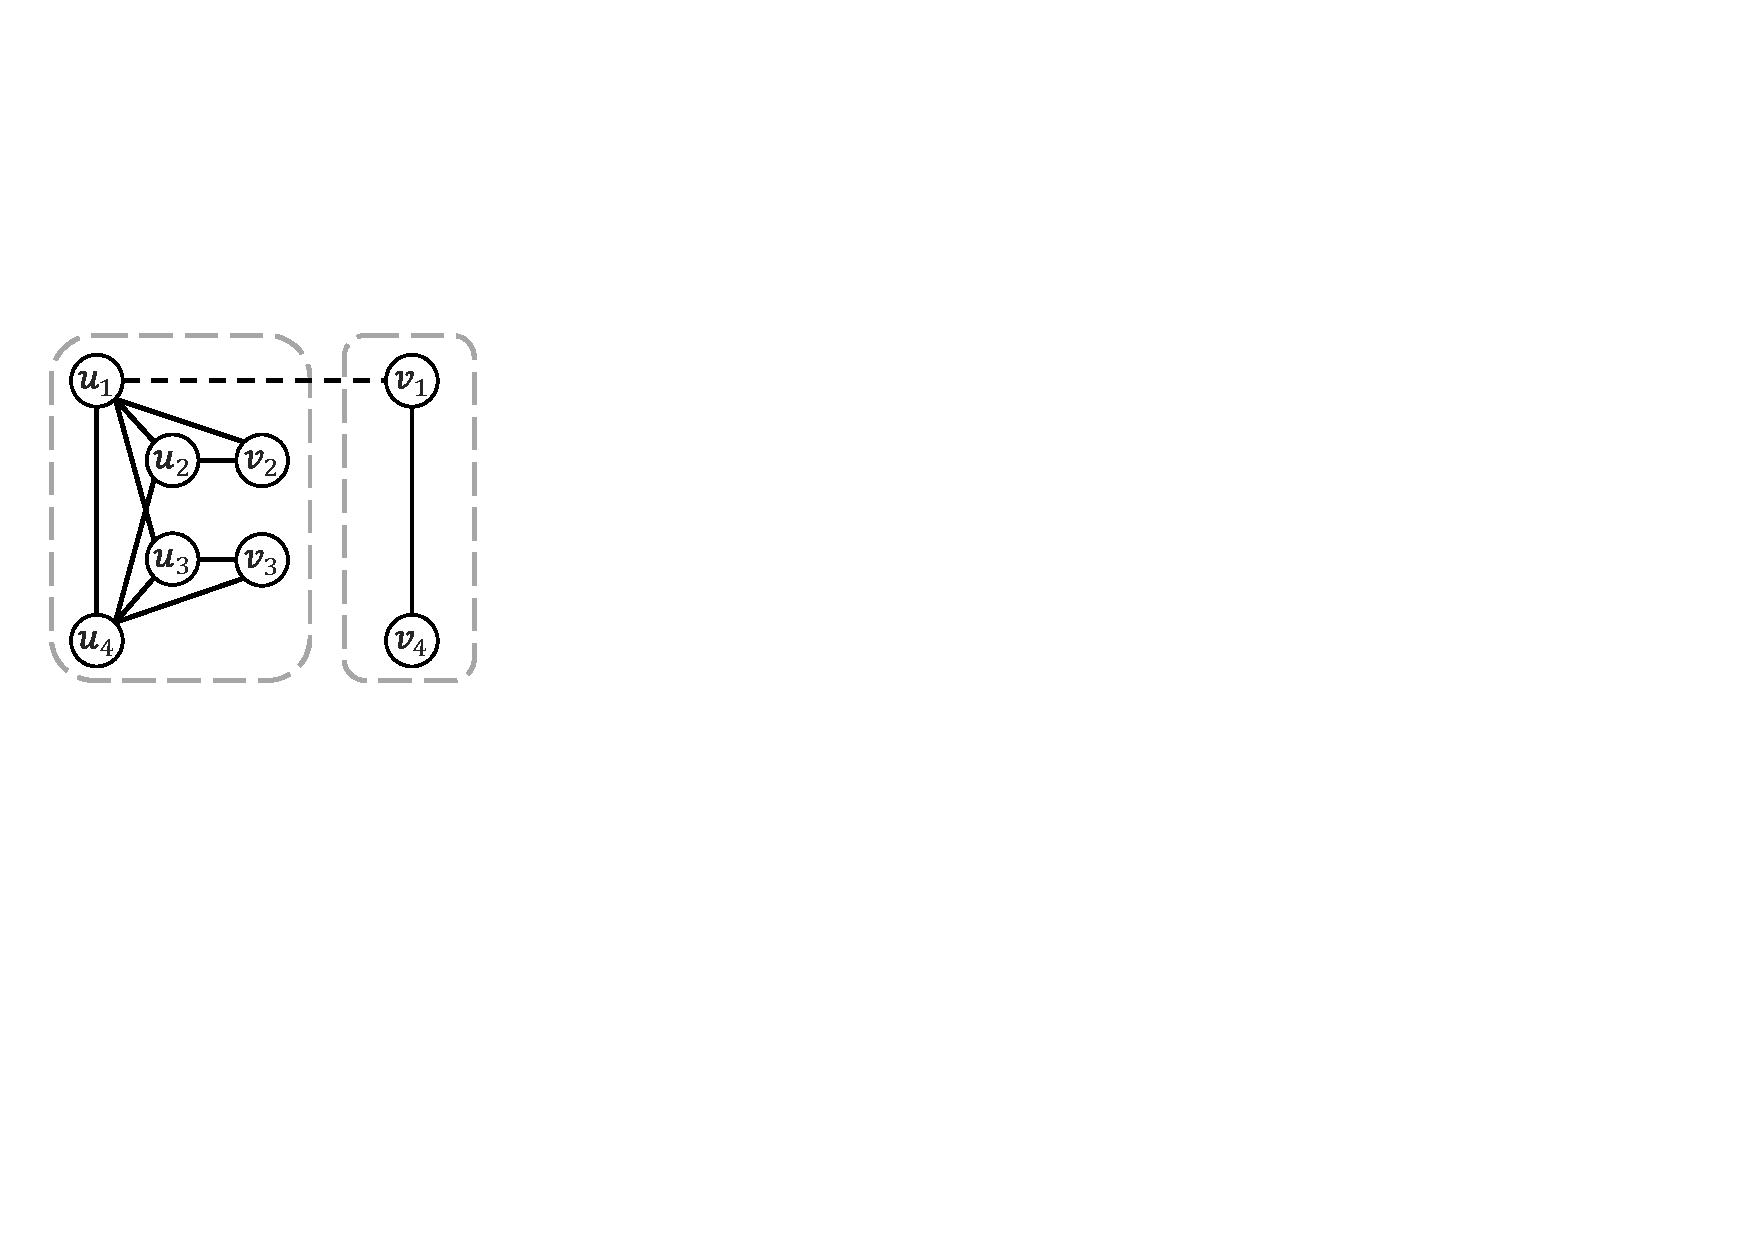
\includegraphics[width=0.8\linewidth]{figures/challenge_partition_a.pdf}
            \end{subfigure}
         \caption{点划分示意图。}
        \label{fig:challenge_partition_vertex}
    \end{figure}

    \item 边划分。和点划分的定义类似,边划分以边作为划分单元,分配到不同的机器上。不同的是,一个点的边可能出现在多台机器上,称之为割点,因此无法采用传统的点对点同步方式,而是将其中一个点设为实际存储点,而将其他点作为镜像点,每次同步时镜像点和实际存储点之间进行同步操作。如图~\ref{fig:challenge_partition_edge}所示,点 $v_1$ 就是一个割点。边划分的目标是尽量减少割点的数量。
    
    \begin{figure}[h]
        \centering
            \begin{subfigure}{0.6\linewidth}
                \centering
                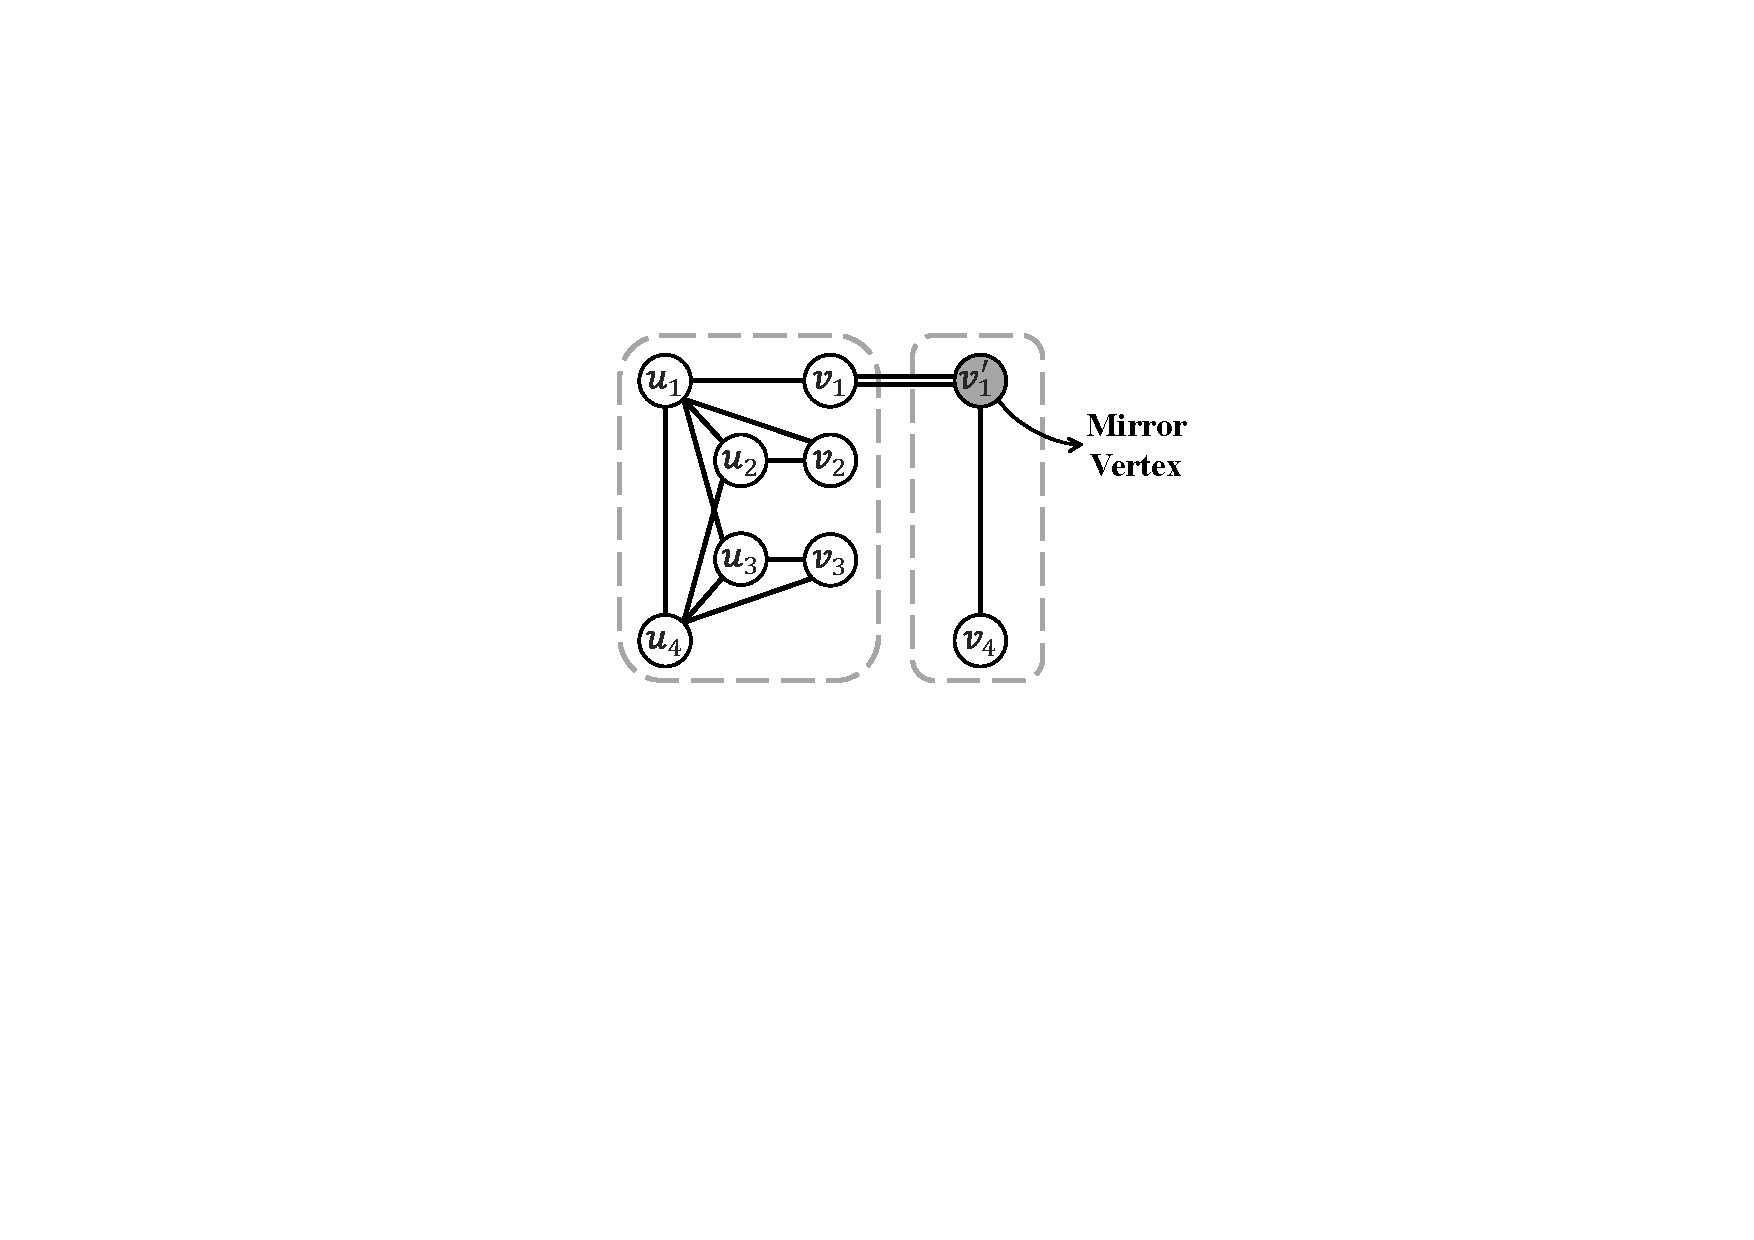
\includegraphics[width=0.8\linewidth]{figures/challenge_partition_b.pdf}
            \end{subfigure}
         \caption{边划分示意图。}
        \label{fig:challenge_partition_edge}
    \end{figure}
    
    \item 混合划分。注意到点划分和边划分都很容易引起负载均衡问题。一个割边或割点较少的划分并不意味子图的大小时平衡的,例如图~\ref{fig:challenge_partition_vertex}和图~\ref{fig:challenge_partition_edge}中的子图大小相差过大。为了解决这一问题,混合划分集成了点划分的思路,但不再以割边为衡量目标,而是综合考虑各种参数,例如节点的度数、节点的连通度、节点的计算量等,直接量化估计整体的划分质量。图~\ref{fig:challenge_partition_hybrid}是一个优化后的划分,虽然存在三条割边,但是八个节点均匀的分配到两个子图中。
    
    \begin{figure}[h]
        \centering
            \begin{subfigure}{0.4\linewidth}
                \centering
                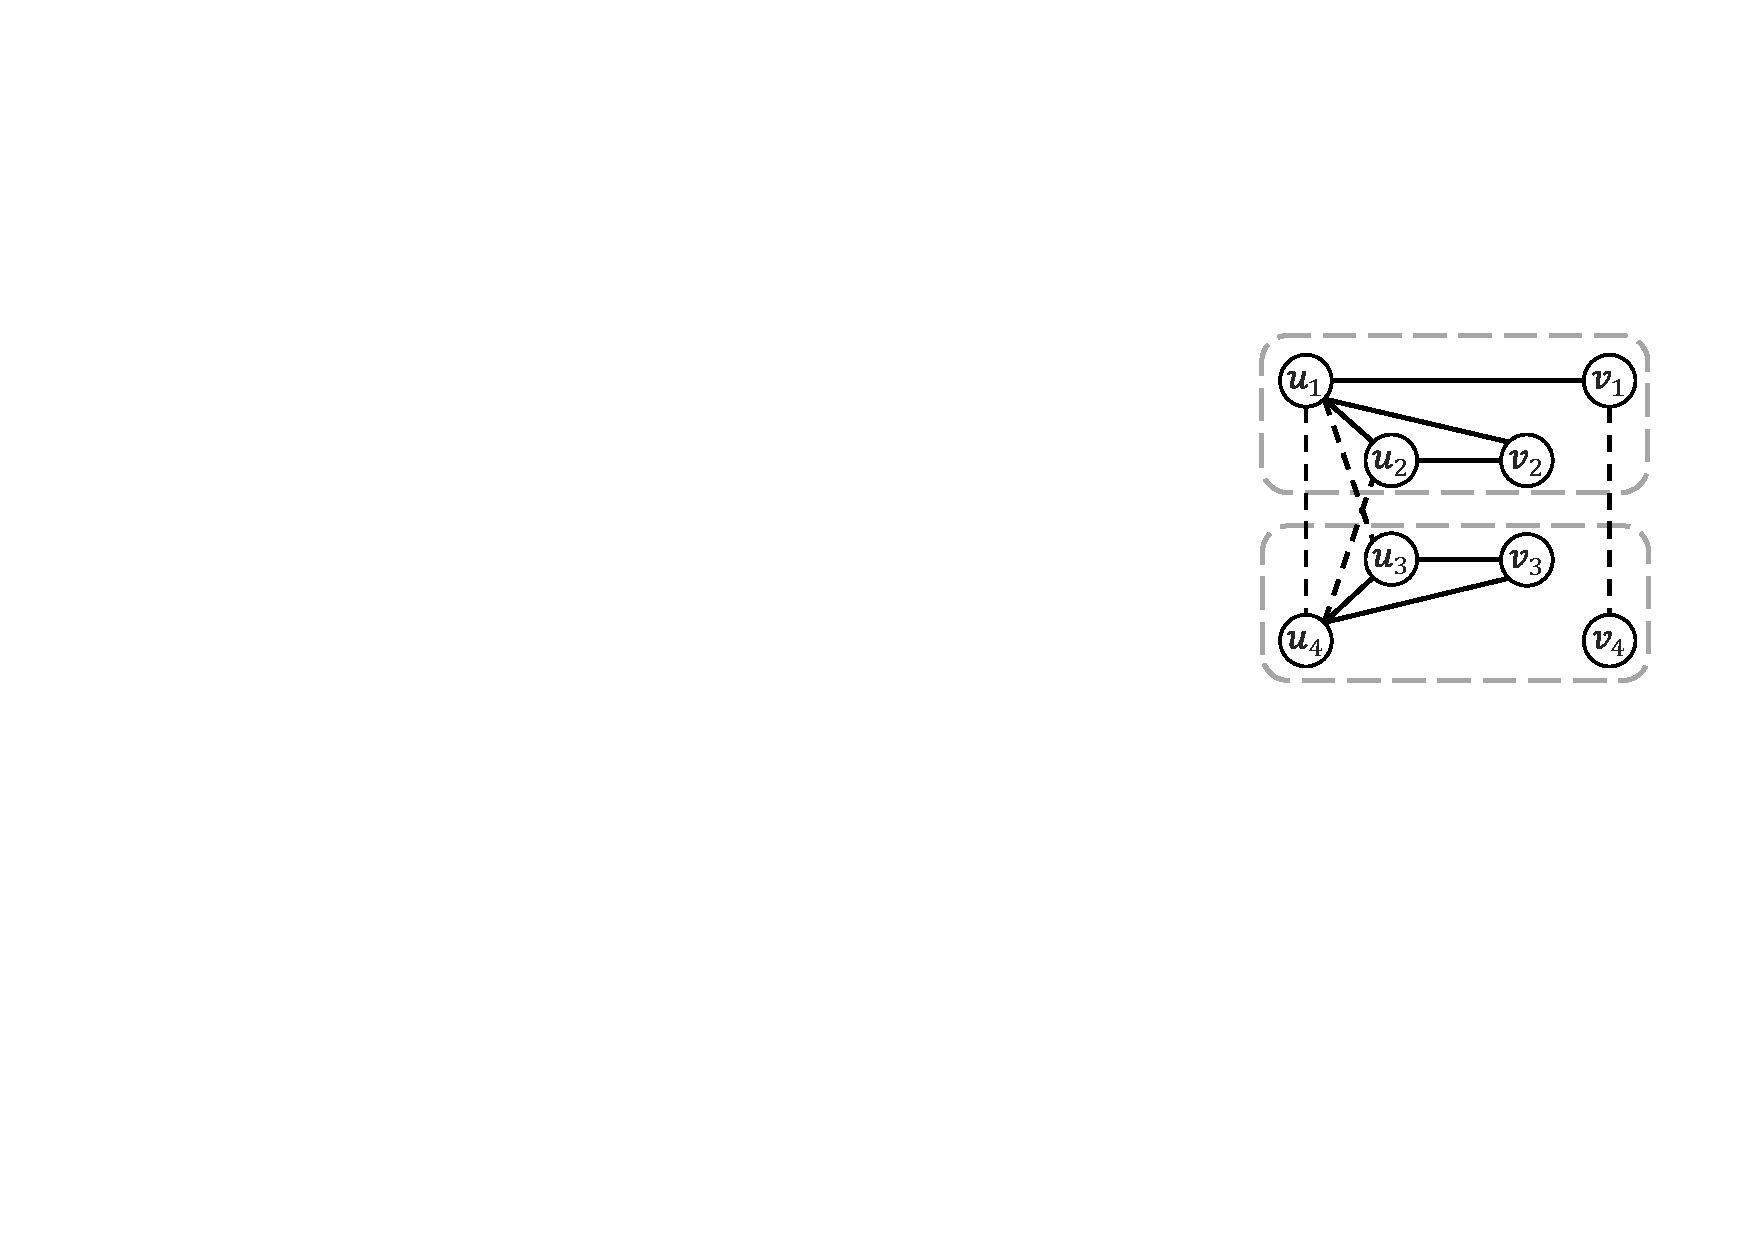
\includegraphics[width=0.8\linewidth]{figures/challenge_partition_c.pdf}
            \end{subfigure}
         \caption{混合划分示意图。}
        \label{fig:challenge_partition_hybrid}
    \end{figure}

\end{itemize}



\section{分布式图计算的计算模式}
\label{sec:distribution_model}

目前,主流的图计算模式都依赖于块同步并行模型(Bulk Synchronous Parallelism,BSP)。BSP模型的思想是将计算任务分为多个超步,每个超步包含以下三个阶段:

\begin{itemize}
    \item 本地计算。每个线程独立地处理自己的计算任务,并且只能用本地存储的数据,无法和其他线程交互。
    \item 通讯。完成本地计算后,线程之间允许通过特定的通讯方式交换数据,并保存为本地数据,用于下一轮本地计算。
    \item 同步。同步操作用于确保所有的线程在完成了当前超步本地计算和通讯操作之后才能进入下一个超步,确保数据一致性。如果没有同步操作,就会出现部分线程读取到了旧数据,导致答案收敛变慢甚至出错。
\end{itemize}

BSP模型将复杂的并行计算拆解成了三个步骤,并且各个阶段所需的计算资源不同:本地计算依赖于计算效率;通讯依赖于通讯的速度和带宽;同步则依赖于负载的均衡。从这三个维度入手,就可以清晰地看出某个特定的计算任务的瓶颈。

在图计算系统中,这三个步骤一般会被抽象为相关的接口函数,用户只需重载本地计算和通讯的代码,图计算系统会自动完成其他剩余的任务,例如图划分、通讯协议、同步信号等等,给用户带来了便利的编程体验。目前,主流的图计算模式分为以下几种:以点为中心、以边为中心、以块为中心、以子图为中心。

\subsection{以点为中心的计算模式}

以点为中心(Vertex-Centric)的计算模式是最基本也是最直观的计算模式。这种模型强调将图中的每个节点视为独立的计算单元,每个节点不仅能够在其内部执行特定的本地计算任务,还可以与其他节点通讯交换信息。这一设计理念极大地简化了复杂图算法的设计过程,允许用户专注于单个节点的行为逻辑,而不需要管理整个图的并发控制细节,尤其是本身就定义在节点上的算法,能够非常自然的迁移到以点为中心的计算模式上。

在以点为中心的计算模式中,用户的职责被简化为定义一个基于点的计算接口,该接口描述了每个点如何处理其状态更新以及如何向相邻节点发送消息。随后,底层平台会负责在整个图的所有节点上并行执行这个接口,可以设定固定的迭代次数或者直到系统达到稳定状态(即收敛)。这种方法不仅提高了开发效率,还增强了代码的可读性和维护性。例如,下述伪代码展示了如何实现最短路径的Bellman-Ford算法:
\begin{lstlisting}
compute(vertex u):
    for m in messages:          # 更新当前的最短路径
        u.dist = min(u.dist, m)
    for [u, v, w] in edges[u]:  # 发送当前的最短路径
        send_message(v, u.dist + w)
\end{lstlisting}
其中dist数组和edges数组存储在本地,用于记录当前的最短路径距离和出边;messages是一个保留字,用于存储上一轮通讯中收到的数据;send\_message也是一个保留字,用于向特定的节点发送数据,并保存在对应的messages中。
该代码分为两部分,首先每个节点根据上一轮收到的最短路径更新自身的最短路径;然后遍历所有的边,构成新的可能的最短路径并发送给对应的节点。执行完该代码后,视作完成了一个超步,由计算平台负责同步。

在这个例子中可以看到,这些计算模式可以大大简化用户层面的编程难度。此外,也有一些计算平台进一步扩展更高级的接口,例如将计算和通讯拆分成两个不同的函数Scatter和Gather,能够更好地对两个阶段单独优化。
\begin{lstlisting}
Scatter(vertex u):
    for [u, v, w] in edges[u]:  # 发送当前的最短路径
        send_message(v, u.dist + w)

Gather(vertex u):
    for m in messages:          # 更新当前的最短路径
        u.dist = min(u.dist, m)
\end{lstlisting}

此外,在多机多线线程的环境下,为了减少机器之间的通讯量,可以提前对数据进行聚合操作,即如果出现了多个发往同一节点的最短路径,可以直接筛选出最优的那一个。
\begin{lstlisting}
Combine(target v, message m1, message m2):
    return min(m1, m2)
\end{lstlisting}

目前,70\%以上的工作都是基于以点为中心的计算模式完成的,这是最广泛的计算模式。然而,以点为中心的计算模式最大的缺点是负载均衡不佳,每一次同步时都需要等待所有线程完成后才能进入下一个超步。且在一些呈现幂律分布的图中,少量度数极大的节点会产生大量的通讯。

\subsection{以边为中心的计算模式}

注意到虽然在每个节点上的计算量往往会受到度数的影响而导致负载不均衡,但是在单条边上的计算量往往是恒定的,因此以边为中心的计算模式就是以边为调度单位。同样以最短路径举例,每条边只需要用起点的距离更新终点即可。
\begin{lstlisting}
compute(edge [u, v, w]):        # 更新当前的最短路径
    update(v', u.dist + w)          
\end{lstlisting}
由于以边为中心的计算模式存储的是完整的边,即采用了边划分的划分算法,因此可以每台机器各自的$v'$上实时更新,并在同步阶段和其他机器同步即可。此时用户只需要关注于本地计算阶段。

此外,同样有一些平台给出了细粒度更高的接口,允许用户分开定义计算操作,并且允许用户自定义是否激活节点,例如GAS模式:
\begin{lstlisting}
Gather(edge [u, v, w]):         # 所有边计算出边的最短路径
    return u.dist + w

Sum(distance dist1, distance dist2):    # 合并相同终点的最短路径
    return min(dist1, dist2)

Apply(vertex u, distance dist): # 所有点更新最短路径
    u.dist = min(u.dist, dist)

Scatter(edge [u, v, w]):        # 如果最短路径发生变化,激活邻居
    if u.dist changed:
        activate(v)
\end{lstlisting}
Gather函数统一负责计算需要更新的值,并且通过Sum函数聚合,减少通讯;Apply函数更新值;Scatter函数用于判断结果是否收敛。在这里,Gather函数和Scatter函数都是定义在边上的,并且边划分可以非常方便地在本地设置镜像点,向用户隐藏了同步细节,而像是在一张完整的图上进行计算。然而,以边为中心的计算模式最大的缺点在于只能在邻居之间传递消息,无法和其他点通讯。

\subsection{以块为中心的计算模式}

以块为中心的计算模式则是更进一步,直接将图划分为多个互不相交的子图并进行计算。在计算阶段,块内部可以采用任意算法计算,只需要在同步阶段同步一轮数据即可。
\begin{lstlisting}
compute(block b):               # 计算块内部的最短路径
    compute shortest path in b
\end{lstlisting}

以块为中心的计算模式特别适用于解决最短路径这种有顺序要求的问题,因为在以点和以边为中心的计算模式中,最短路径算法的同步次数与图的直径相关,即至多需要直径轮才能将最短路径传播到所有节点。然而在以块为中心的计算模式中,由于块内部可以采用Dijkstra算法或SPFA算法等串行算法快速计算,减少了直径对执行时间的影响。

\subsection{以子图为中心的计算模式}

上述所有计算模式均无法较好的解决模式匹配问题,例如计算图中有多少个四阶完全图,一方面计算子图需要大量的通讯以同步邻居信息,另一方面模式的数量无法良好估计,也会产生严重的负载不均衡。

以子图为中心的计算模式则是尝试直接构造子图,并以子图为单位进行调度。它和以点为中心的计算模式类似,都是从每个节点触发尝试构造子图,而后续则是直接以子图作为任务调度的单位,尝试在原图中拉取邻居生成子图,并统计模式数量。
\begin{lstlisting}
pre_compute(vertex u):          # 生成初始子图,仅包含一个点
    sg = [[u], []]
    subgraph.push_back([u])

compute(subgraph sg):
    u = sg.vertex[0]            # 获取初始子图对应的节点
    sg.add(pull(u))             # 获取邻居,并加入子图
    count(sg)                   # 在子图上统计具体的模式数量
\end{lstlisting}



\section{常见图计算平台上的最短路径算法实现}
\label{sec:distribution_algorithm}

由于各个图计算平台的接口各不相同,各自的实现方式也有很大差异,因此下面会给出一些常见的计算平台的基本介绍,以及这些计算平台上的最短路径算法实现。

\subsection{GraphX平台}

GraphX 是 Apache Spark上的一个分布式图处理框架,它使得用户能够在大规模图数据集上执行高效的图计算。GraphX 结合了 Spark 的强大功能,采用了和 Spark 一样的RDD存储结构,能够和已有的数据分析模块相结合,且自带了容错机制和故障处理机制,为用户提供了一个灵活且高性能的图处理解决方案。此外,GraphX还提供了类似于Pregel的接口以提供高效的图计算。

然而,由于Spark本身依赖于JVM,导致GraphX的计算效率较低,并且Spark中的基本数据单元RDD无法直接修改,导致图计算中每次迭代都需要拷贝数据才能实现更新,并且Spark采用hadoop存储数据,直接导致IO瓶颈。

GraphX中的最短路径算法可以通过调用Pregel接口来实现,包含三个用户函数:VertexProgram,SendMessage,MergeMessage。在VertexProgram中,每个节点只需保存最优的路径;在SendMessage中,对于每一条出边,尝试构造一条路径并发送给目标节点。在MergeMessage中,发往同一顶点的最短路径会被合并,以减少通讯量。

注意,虽然这里的SendMessage参数是边,但GraphX依然是以点为中心的计算模式,只是在遍历每个点的出边时调用该函数。

\begin{lstlisting}
VertexProgram(vertex u, distance dist, distance new_dist):
    return min(dist, new_dist)

SendMessage(edge [u, v, w]):
    if u.dist + w < v.dist:
        send_message(v, u.dist + w)

MergeMessage(distance dist1, distance dist2):
    return min(dist1, dist2)
\end{lstlisting}

\subsection{PowerGraph平台}

PowerGraph 是一个高效的分布式图处理系统,设计用于高效地处理大规模图数据。它采用以边为中心的计算模式,特别擅长应对具有幂律分布特性的图(即少数节点拥有大量的连接,而大多数节点只有少量连接),这类图在实际应用中非常常见,例如社交网络、网页链接结构等。

PowerGraph 的执行引擎经过优化,能够在大规模集群上高效地执行图算法。它利用了内存计算的优势,避免使用hadoop导致的IO开销,并通过减少不必要的数据传输来提高性能。

PowerGraph中的最短路径算法可以通过GAS模型实现,包含四个用户函数:Init,Gather,Apply,Scatter。Init函数负责记录上一轮收到的最短路径,且该消息已经经过聚合,也就无需使用Gather函数;Apply函数将该最短路径更新;Scatter函数尝试构造新的最短路径,并激活目标节点更新。
\begin{lstlisting}
Init(vertex u, message m):
    new_dist = m

Gather(edge [u, v, w]):
    return null

Apply(vertex u):
    u.dist = new_dist

Scatter(edge [u, v, w]):
    new_dist = u.dist + w
    if new_dist < v.dist:
        signal(v, new_dist)
\end{lstlisting}






\subsection{Flash平台}

Flash是一个高效的图计算平台,能够同时支持对集合的操作,跨领域的通讯,以及灵活的控制流。Flash平台是Ligra平台的扩展,Ligra仅支持单机多线程,而Flash将其扩展到了多机上。Flash设计了中间层FlashWare来实现高效的通讯、负载均衡、同步、调度等功能,并且只会更新实际需要的属性,避免整个节点的拷贝。整个中间层都是向用户隐藏的,可以自动地在任务中执行而无需用户配置。

Flash相比于Pregel最大的优势是支持针对子集的操作,即可以自由地定义点集和边集并在此基础上执行图算法,而已有的大部分平台仅支持在全图上计算。除了子集,Flash甚至支持扩展集合的操作:例如为了统计矩形(四个节点组成的环)的个数时,可以直接对边集执行join操作,此时$E$ join $E$就代表了两跳邻居,而每一对起终点相同的两跳邻居都能够组成一个矩形。

Flash中的最短路径算法可以通过EdgeMap函数实现,和Pregel类似,对于每个顶点的每条出边,都会调用EdgeMap中的Update函数,用节点 $u$ 的距离更新 $v$ 的距离;不同的是,这里返回的是点$v$的一个拷贝,在Reduce函数中才会真正对比最短路径,并保留最优的一个。这种来自C++语法的自由度给Flash带来了更方便的表达,能够支持更加复杂的语法。而在主函数中,通过while循环不断对激活点集$V$进行扩展,直至收敛。

\begin{lstlisting}
Update(edge [u, v, w]):
    dis[v] = min(dis[v], dis[u] + w)
    return v

Reduce(vertex new_vertex, vertex old_vertex):
    if new_vertex.dist < old_vertex.dist:
        return new_vertex
    else:
        return old_vertex

main():
    while size(V) != 0:
        V = EdgeMap(V, E, Update, Reduce)
\end{lstlisting}


\subsection{Pregel+平台}

Pregel+平台是一个基于Pregel语法的优化版本,旨在优化Pregel的消息传递中高度数节点频繁发送消息所带来的通讯开销。Pregel+主要采用了和边划分类似的镜像法,对于度数较高的顶点,在多台机器中都存放镜像节点,这样所有的消息传递都将在本地进行,只需要将镜像节点同步即可。这种镜像法将边之间可能的大量通讯转移到了机器之间,由于机器的数量一般不会很高,所以镜像节点的同步速度是非常快的。镜像法除了可以减少通讯量,还可以减少由于高度数节点所带来的负载不均衡。

由于Pregel+平台仅在底层优化,而没有改变顶层的接口设计,因此大量基于Pregel的算法可以非常方便地移植到Pregel+平台。Pregel+的核心代码仅包含一个compute函数,这里给出我们的实现:
\begin{lstlisting}
compute(vertex u):
    new_dist = u.dist
    for dist in message:
        if dist < new_dist:
            new_dist = dist
    if new_dist < u.dist:
        u.dist = new_dist
        for [u, v, w] in edges[u]:
            send_message(v, u.dist + w)
\end{lstlisting}

\vspace{-1em}
\subsection{Grape平台}

Grape平台是一个以块为中心的计算平台,专门用于优化最短路径这一类和图的直径直接有关的问题。Grape包含两个用户函数,PartialEvaluation(PEval)和IncrementalComputation(IncEval),分别用于块内的初始化计算,以及经过同步后的增量计算。

以最短路径为例,PEval函数负责在块内部调用Dijkstra算法计算当前的最短路径,即仅用当前块内的边能组合出的最短路径:
\begin{lstlisting}
PEval(vertex_set V, edge_set E):
    dist[source] = 0
    initialize PQ as a priority queue
    PQ.push(source, 0)
    while PQ is not empty:
        u = PQ.pop()
        for [u, v, w] in E:
            if dist[u] + w < dist[v]:
                dist[v] = dist[u] + w
                PQ.push(v, dist[v])
    initialize M as a set
    for v in V:
        M.push([v, dist[v]])
    return M
\end{lstlisting}

接下来,Grape会不断调用IncEval直至收敛。具体来说,每个块会收到来自其他块的最短路径,然后尝试用这些最短路径进行松弛操作:
\begin{lstlisting}
IncEval(vertex_set V, edge_set E, message M):
    initialize PQ as a priority queue
    for [v, dist[v]] in M:
        PQ.push(v, dist[v])
    while PQ is not empty:
        u = PQ.pop()
        for [u, v, w] in E:
            if dist[u] + w < dist[v]:
                dist[v] = dist[u] + w
                PQ.push(v, dist[v])
    initialize M as a set
    for v in V:
        M.push([v, dist[v]])
    return M
\end{lstlisting}

Grape这种以块为中心的计算模式介于Dijkstra算法和Bellman-Ford算法之间:前者通过最优性保证每个节点只会被计算一次,而后者则由于自由的计算顺序导致最坏情况下会产生大量重复计算。Grape算法在块内部保证最优,但是块之间的同步会产生一定的重复计算。具体来说,如果一条最短路径穿越了 $k$ 次块边界,那么这条最短路径就需要 $k$ 个超步才能会被计算到。

当然,以块为中心的计算模式最大的意义是给了一些难以并行的顺序算法一种通用的并行可能,即只需要满足增量更新的特点就可以实现并行。



\section{分布式环境下的最短路径算法效率}
\label{sec:distribution2}

在这一章中,我们会将所有平台中的最短路径算法进行测试,以观察不同模式和不同平台下的计算效率差异。

\subsection{测试环境}

所有的实验均在一个高性能计算集群上执行,该集群由16台独立的物理机组成,提供了强大的并行计算能力。每台物理机含有四颗Intel$^\circledR$ Xeon$^\circledR$ Platinum 8163 @ 2.50GHz处理器,每颗处理器包含24个物理核心和48个线程,确保并行计算能力。

此外,考虑到不同的计算平台有不同的存储架构(基于内存或基于磁盘),每台物理器还配备了512GB的DDR4内存和3TB的硬盘空间(通过Hadoop组成存储集群),避免由于内存或硬盘空间不足导致的性能瓶颈。

为了保证各物理机之间的高效通信,这16台机器通过一个带宽为15Gbps的高速局域网相互连接。这种高带宽的网络环境对于分布式计算任务至关重要,尤其是那些需要大量数据通讯的平台。另一方面,带宽不可能无限增大,15Gbps是一个较为合理的数值。

综上所述,这样一个配置完整的集群环境,能够同时满足大规模图数据分析所需的计算资源、存储资源和通讯资源,尽可能减少由于硬件问题所带来的差异,充分发挥出各个平台的设计性能。

\subsection{测试数据集}

为了尽量减少数据集对测试结果的影响,并确保实验结果的可靠性和可重复性,我们采取了一种系统化的方法来生成多样化且可控的人工合成数据集。这些数据集不仅在规模上有所区别,还涵盖了不同的图特征,以便全面评估算法在各种情况下的性能表现。

数据集的生成基于Facebook的社交网络分布,通过学习该网络的节点特征,我们生成了一系列数据集,这些数据集满足社交网络的幂律分布,即少量节点有着较高的度数,且满足小世界定理,即任意两个人之间的最短路径跳数不超过六。

数据集的命名包含规模和特征两部分。数据集的规模是通过其点数和边数来定义的,具体来说,假设图中由 $n$ 个点和 $m$ 条边,该数据集的规模参数定义为点数和边数之和以10为底的对数,即:
\begin{equation*}
    Scale = \log_{10}(n + m)
\end{equation*}
考虑到社交网络图的边数远大于点数,可以近似认为数据集的规模参数是边数的对数。

除此之外,我们还为数据集在两个参数上进行增强,包括:
\begin{itemize}
    \item 稠密数据集。稠密数据集在边数不变的基础上减少了点数,使得密度增大了十倍。这模拟了现实世界中的社交网络或紧密合作的专业社区等场景,在这些环境中,个体之间存在着大量的直接联系。
    \item 大直径数据集。大直径数据集在图规模不变的基础上大大增加了直径,这意味着从起点出发需要更多的超步才能到终点。这对最短路径算法是一个巨大的挑战。
\end{itemize}

\begin{table}[h]\centering
    \def\arraystretch{1.5}
	\caption{生成数据集及其参数}
	\label{tab:syn_data}
	% \small
	\begin{tabular}{c|c|c|c|c}
        % {0.47\textwidth}{>{\centering\arraybackslash}c|>{\centering\arraybackslash}X|>{\centering\arraybackslash}X|>{\centering\arraybackslash}c|>{\centering\arraybackslash}X}
		\hline
		数据集 & 点数 & 边数 & 密度 & 直径 \\ \hline \hline
		S8-Std            & 3.6M       & 153M       & $2.4 \times 10^{-5}$     & 6                           \\ \hline
		S8-Dense          & 1.2M       & 159M       & $2.2 \times 10^{-4}$     & 5                           \\ \hline
		S8-Diam           & 3.6M       & 155M       & $2.4 \times 10^{-5}$     & 101                         \\ \hline
		S9-Std            & 27.2M      & 1.42B      & $3.8 \times 10^{-6}$     & 6          \\ \hline
		S9-Dense          & 9.1M       & 1.47B      & $3.6 \times 10^{-5}$     & 5                            \\ \hline
        \ \ \ \ \ S9-Diam   \ \ \ \ \  &  \ \ \ \ \ 27.2M \ \ \ \ \      &  \ \ \ \ \ 1.48B  \ \ \ \ \ &  \ \ \ \ \ $4.0 \times 10^{-6}$  \ \ \ \ \ &  \ \ \ \ \ 102   \ \ \ \ \  \\ \hline
	\end{tabular}
\end{table}


\subsection{运行时间的对比}

首先,我们在单机32线程下对比各个平台执行最短路径的时间,减少由于通讯所带来的影响。这种设置允许我们专注于算法本身的效率,而不必担心分布式环境中常见的网络延迟和其他通信开销。具体结果如图~\ref{C9-fig1}所示。

从三个数据集对比来看,大直径数据集所花费的时间远远多于其他两个数据集,这也和之前的理论分析相符合,即最短路径算法的执行时间受到图的直径影响,图的直径越多,计算平台就需要更多的超步执行,而每个超级步都需要同步操作,这些同步点会引入额外的等待时间,从而导致总体执行时间增加。另一方面,高密度的数据集显示出更短的执行时间。尽管稠密图中的点数较少,且每个节点有更多的邻居,但相关的计算可以更加集中和高效地进行,这种集中性减少了冗余计算,提高了处理速度。

从六个平台对比来看,Grape和Ligra展现出了最快的执行速度,因为Grape就是为了解决最短路径问题之类顺序算法而设计的,使其在解决这类问题时表现出色,而Ligra的轻量级设计也让它在单机环境下能够快速响应并高效处理任务,因此它的执行速度也非常快;PowerGraph、Flash和Pregel+运行速度其次,但在大多数情况下仍能提供合理的执行时间;GraphX是最慢的平台,这一结果主要归因于 Spark 平台自身的限制,包括较高的启动延迟、JVM 堆栈管理开销以及序列化/反序列化的成本等。

\begin{figure}[h]\centering
    \begin{subfigure}[b]{0.7\textwidth}
        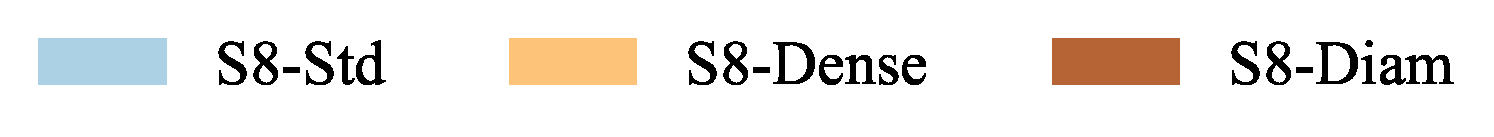
\includegraphics[width=\textwidth]{figures/legend_horizontal.pdf}
    \end{subfigure}

    \begin{subfigure}[b]{0.8\textwidth}
		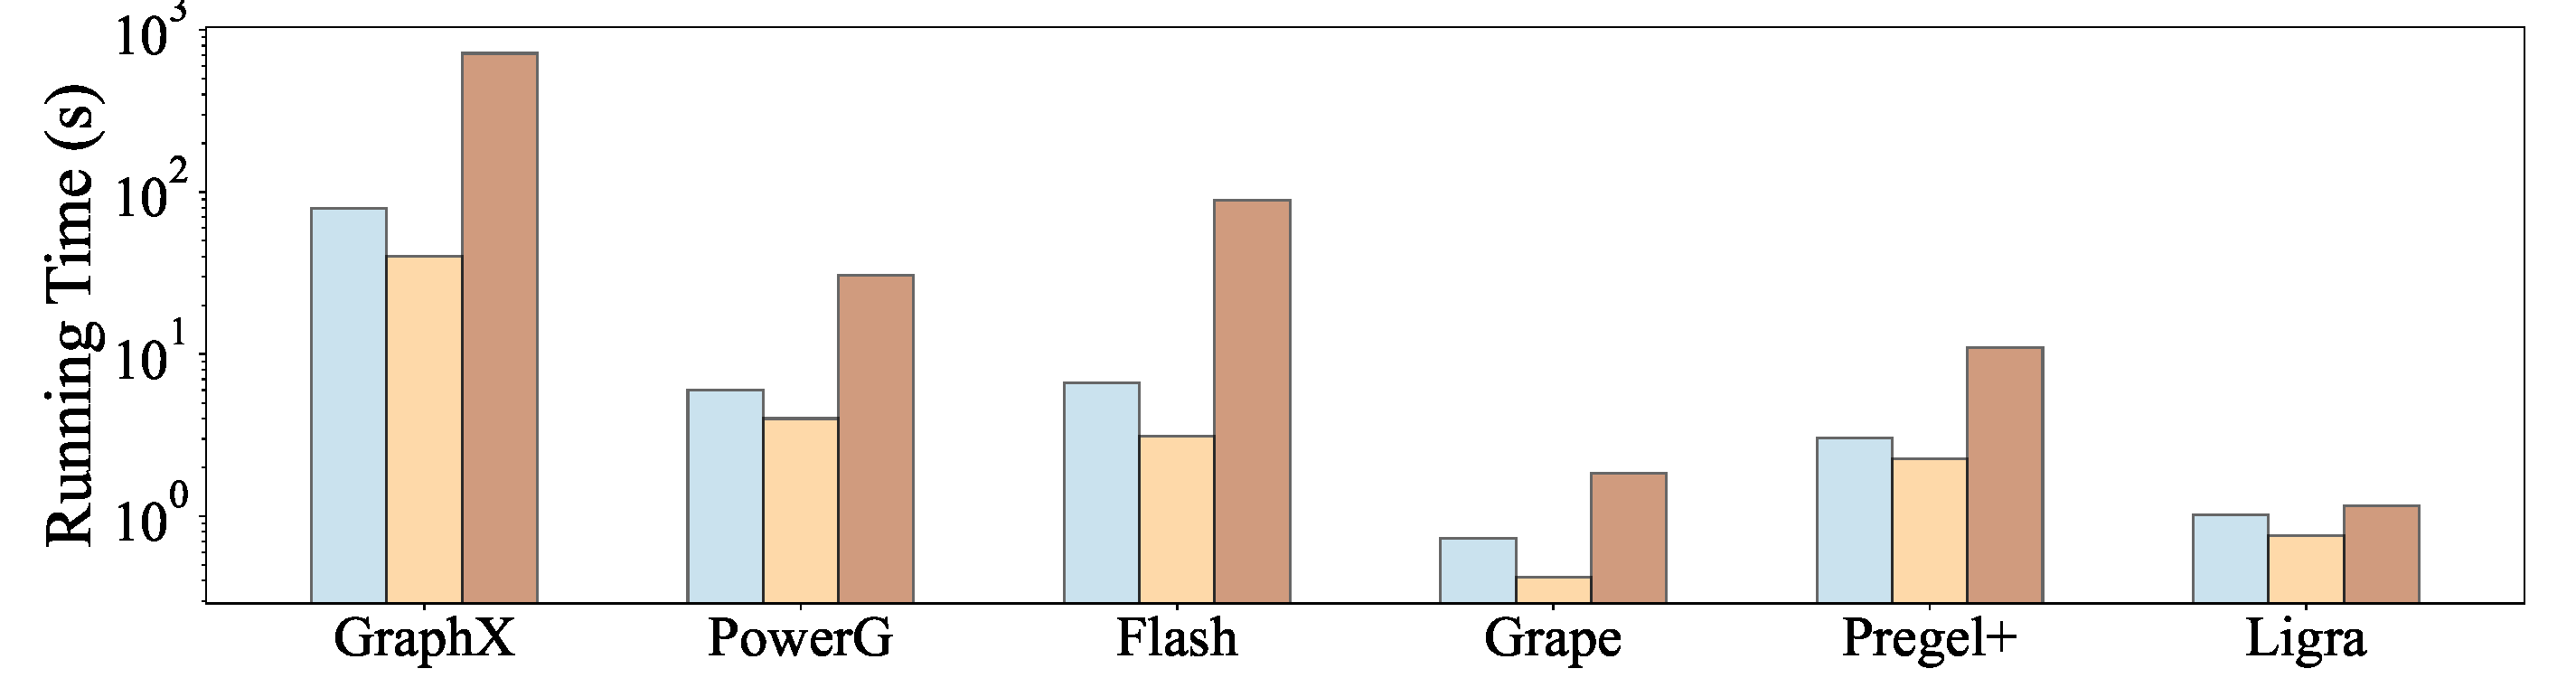
\includegraphics[width=\textwidth]{figures/algorithm-sensitivity-SSSP.pdf}
	\end{subfigure}
    \caption{六个分布式计算平台下的三个不同数据集的最短路径算法执行时间。}
    \label{C9-fig1}
\end{figure}

\subsection{扩展性的对比}

为了全面评估图计算平台的扩展性,我们进行了详细的实验设计,分别测试了在不断增加线程数量(纵向扩展性)和不断增加机器数量(横向扩展性)情况下的运行时间变化。这些实验不仅帮助我们理解系统如何应对不同的计算资源配置,还揭示了影响其性能的关键因素。

纵向扩展性指的是通过增加单台机器的计算资源来提高其处理能力,在本实验中,即通过增加单机上的线程数量来进行测试。这种方法主要关注的是系统本身的计算性能以及算法的优化能力。一方面,纵向扩展性测试帮助我们了解平台如何有效地利用多核处理器的能力;另一方面,纵向扩展性测试体现了算法的并行程度以及在算法实现上的优化水平。这种设置允许我们专注于系统和算法本身的效率,而不必担心分布式环境中常见的网络延迟和其他通信开销。

与纵向扩展性相对应,横向扩展性是指通过增加机器数量来提高整个系统的计算能力。在本实验中,即通过逐步增加参与计算的机器数量来进行测试。这种方法更加考验系统设计的能力,尤其是当增加机器数量时,有效地分配任务以确保各个节点之间的负载均衡,以及优化通信机制,选择合适的通信协议和拓扑结构,减少不必要的数据传输。

通过这种方式,我们可以更清晰地识别出哪些因素是限制系统性能的关键所在,并为后续的优化提供方向。

\subsubsection{纵向扩展性的对比}

纵向扩展性指的是在一台机器中增加线程所带来的加速。我们在单机上使用1、2、4、8、16、32线程进行测试,其中GraphX至少需要2线程才能成功执行。

图~\ref{fig:exp_scalability_threads} 展示了不同线程数量下的最短路径算法执行时间,所有平台都展现出良好的纵向扩展性,即随着线程的增多,执行时间显著下降。详细的加速倍数,即最佳性能与单线程性能的比率,在表~\ref{tab:exp_scalability_threads}中列出。

\begin{table}[h]\centering
    \def\arraystretch{1.5}
    \caption{纵向扩展性加速倍数}
    \label{tab:exp_scalability_threads}
    \tiny
    \resizebox{0.9\linewidth}{!}{
    \begin{tabular}{c|c|c|c|c|c|c}
    \hline
        Dataset   &  GraphX  &  PowerG  &  Flash &  Grape  &  Pregel+  &  Ligra  \\ \hline\hline
        S8-Std      & 6.9    & 5.0    & 9.3   & 23.5  & 8.8     & 2.0   \\
        S8-Dense    & 7.8    & 5.8    & 8.5   & 19.7  & 11.3    & 2.4   \\
        S8-Diam     & 6.7    & 0.9    & 10.2  & 13.2  & 10.1    & 1.8   \\ \hline
    \end{tabular}
    }
\end{table}

\begin{figure}[h]\centering

	\scalebox{0.35}[0.35]{
\includegraphics{figures/vertical_scalability_legend.pdf}}

	\begin{subfigure}[b]{0.8\textwidth}
        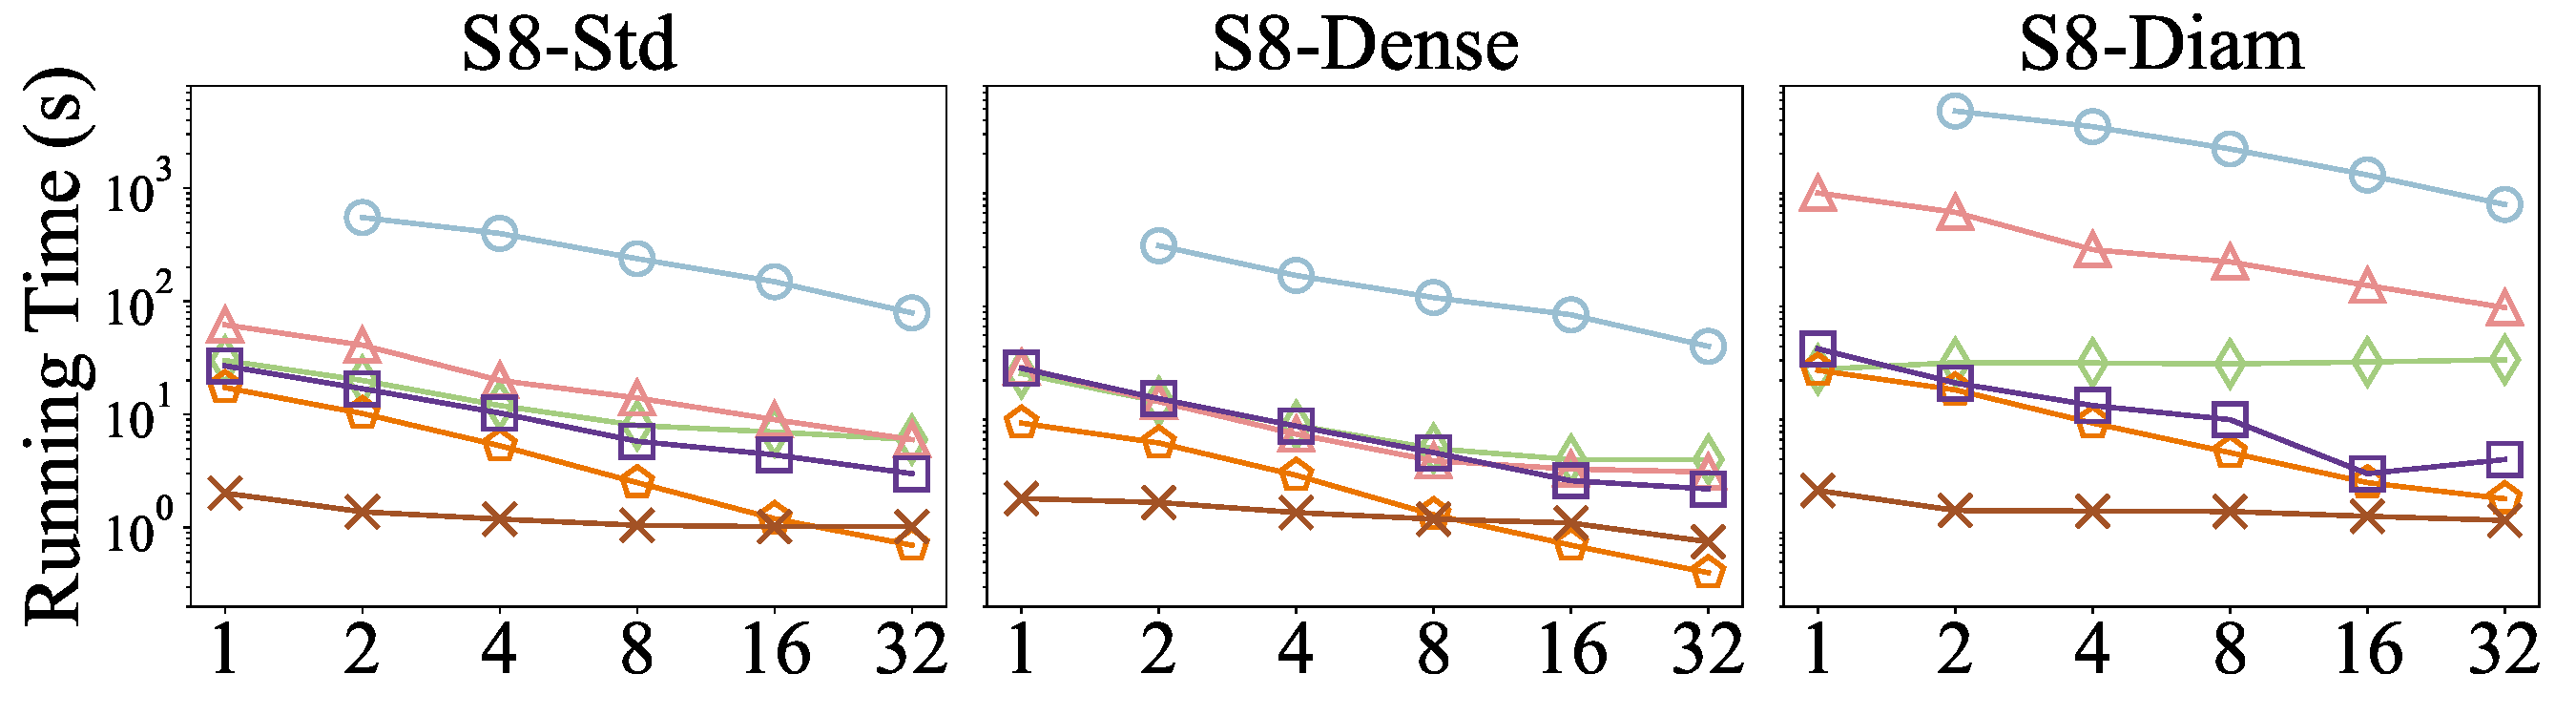
\includegraphics[width=\textwidth]{figures/sssp_vertical_scalability.pdf}
    \end{subfigure}
	
	\caption{在单机不同线程数量下的最短路径算法执行时间。}
	\label{fig:exp_scalability_threads}
\end{figure}

整体来看,Grape展现出较好的纵向扩展性,最高可达23倍,其次是Pregel+、Flash、GraphX和PowerGraph,平均约为5$\sim$10倍。特别地,Ligra的纵向扩展性较差,这可能是因为Ligra平台本身的速度很快,而预处理时间由占据了较多的一部分,导致加速不明显。

从三个数据集来看,纵向扩展性在不同特性的数据集上也有很多差异。大多数平台在稠密数据集上有着更好的纵向扩展性,这是因为随着密度的增加,计算也会更加集中在更少的点上。然而,在大直径数据集上的扩展性一般较差,甚至PowerGraph平台呈现出负收益,这可能是由于超步数量快速增加而导致的。


\subsubsection{横向扩展性的对比}

横向扩展性指的是增加机器数量所带来的加速。我们在1、2、4、8、16台机器上进行测试,每台机器都使用了32线程。由于计算资源成倍增加,我们选用更大的数据集进行测试。其中GraphX无法在S9-Diam上完成计算,且至少需要4机才能在其他两个数据集上完成计算;Ligra由于仅支持单机,所以没有被包含在实验内。

图~\ref{fig:exp_scalability_machines_9} 展示了不同机器数量下的最短路径算法执行时间,可以看到横向扩展性对比纵向扩展性较为一般,但随着机器的增多,执行时间整体呈现下降趋势。详细的加速倍数,即最佳性能与单机性能的比率,在表~\ref{tab:exp_scalability_machines}中列出。

\begin{table}[h]\centering
    \def\arraystretch{1.5}
   \caption{横向扩展性加速倍数}
   \label{tab:exp_scalability_machines}
   \tiny
   \resizebox{0.8\linewidth}{!}{
	   \begin{tabular}{c|c|c|c|c|c}
		   \hline
		   Dataset   &  GraphX  &  PowerG  &  Flash &  Grape  &  Pregel+   \\ \hline \hline
		   S9-Std      & 1.8    & 2.6    & 1.2   & 1.7   & 2.4   \\
		   S9-Dense    & 2.2    & 2.9    & 1.3   & 3.3   & 3.1   \\
		   S9-Diam     & ---    & 1.4    & 2.0   & 0.5   & 4.0   \\ \hline
	   \end{tabular}
   }
\end{table}

\begin{figure}[h]\centering

    \scalebox{0.35}[0.35]{
\includegraphics{figures/vertical_scalability_legend.pdf}}
    
    \begin{subfigure}[b]{0.8\textwidth}
        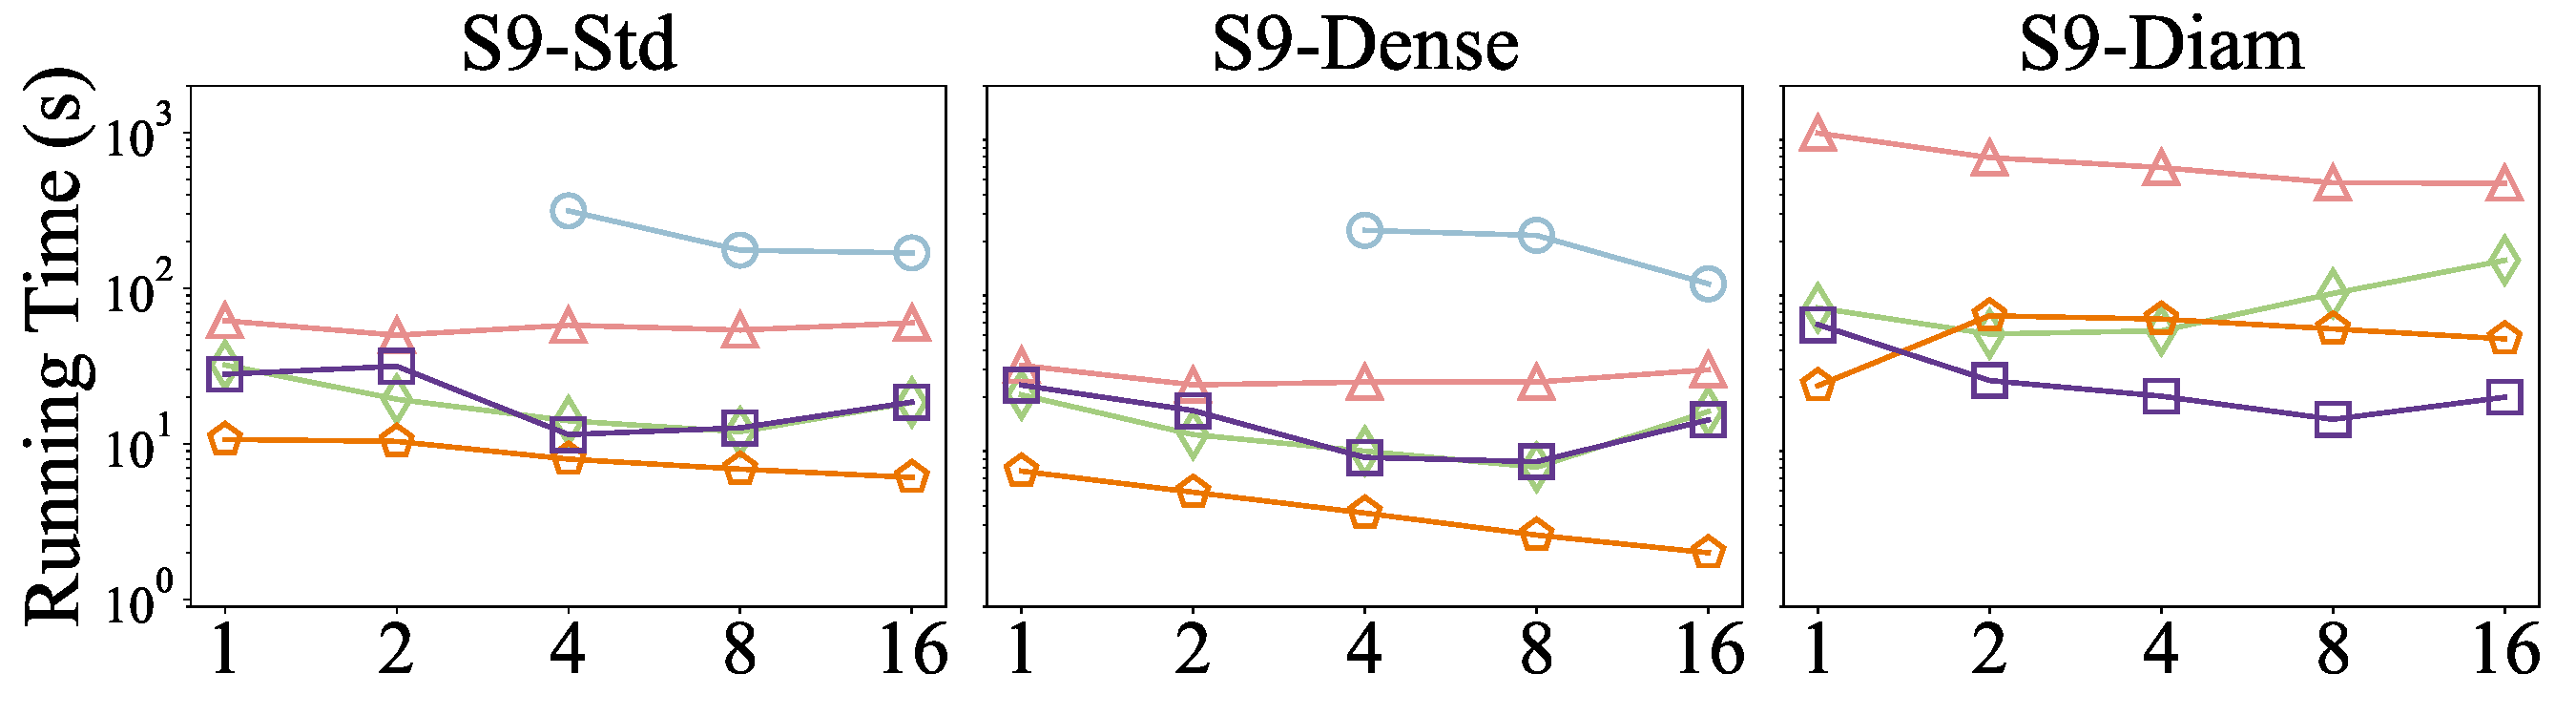
\includegraphics[width=\textwidth]{figures/sssp_horizontal_scalability_9.pdf}
    \end{subfigure}

    \caption{在不同机器数量下的最短路径算法执行时间。}
    \label{fig:exp_scalability_machines_9}
\end{figure}

所有平台的横向扩展性相比纵向扩展性都较差,这可能是由于机器间通信的巨大开销所致。此外,大部分平台在单机上已经已经实现了非常好的性能,扩展到多台机器时,由于不可避免的通信开销,其性能增益趋于饱和。

而在不同数据集上的横向扩展性和纵向扩展性都较为类似,即在稠密数据集上表现更好,而在大直径数据集上表现较差,甚至同样会呈现出负收益。

\subsection{平台性能对比与选取参考}

从以上运行时间和扩展性对比的实验可以看出,不同的计算平台之间的差异较为明显,一方面受到平台本身语言和依赖的基础架构限制,另一方面也有本身计算模式之间的优劣,具体来说:
\begin{itemize}
    \item 平台特性的影响。六个平台中除了GraphX使用Scala编写之外,其他平台均选择使用C/C++语言,并使用OpenMPI或MPICH进行通讯,从实验结果也可以看出C系列语言高效的运行速度以及更加自由的编写模式。此外,基于内存存储的平台相比于基于硬盘存储的平台运行速度也有显著的提升,然而,代价是将数据导入内存需要消耗大量的时间,且内存的价格也是不可忽略的一部分。
    \item 计算模式的影响。在本实验中,我们选取的最短路径算法其实是一个比较复杂的问题,因为传统的Dijkstra无法很好的并行化,而经典的以点和边为中心的并行计算模式则只能采用最基础的Bellman-Ford算法,这就意味着虽然并行能够减少实际的运行时间,但是代价却是增加了大量的冗余计算。相比之下,以块为中心的计算模式则更加擅长解决这一类问题。
\end{itemize}
在实际应用中,则需要根据不同的落地需求综合考虑多个因素选取计算平台,包括:
\begin{itemize}
    \item 应用场景。对于大规模的分布式计算,GraphX这种带有全面容错机制的平台显然是最合适的,PowerGraph和Pregel+也在一定程度上提供了容错能力;而对于小规模的快速开发,单机的Ligra则更加合适。
    \item 性能需求。如果对性能有较高的要求,应优先考虑那些在运行时间测试和扩展性测试中表现出色的平台,如Grape和PowerGraph,这些平台提供了极致的性能优化,能够最快地完成计算任务。
    \item 算法需求。由于分布式算法编写难度较高,如果用户需要其他更加复杂的图算法,Flash提供的大量图算法会带来帮助。并且Flash包含了大量在顶级会议上最新发表的高效算法,可以带来更高的效率。
    \item 兼容性需求。在一些情况下需要和已有数据和算法兼容,例如GraphX可以直接对接Spark处理后的数据,Pregel+也可以直接运行Pregel编写的代码,而无需过多的修改。
\end{itemize}